% book of functional analysis exercises
% nicola frosi
% starting date 18-05-2024

\documentclass[a4paper, twoside, openany]{book}

\usepackage[utf8]{inputenc}
\usepackage[T1]{fontenc}
\usepackage[english]{babel}

\usepackage[margin=2.5 cm]{geometry}

\usepackage{float}
\usepackage{rotating}

\usepackage{cancel}

\usepackage{amsmath}
\usepackage{amsfonts}
\usepackage{amssymb}
\usepackage{amsthm}

\usepackage{tikz}
\usetikzlibrary{arrows.meta, calc, quotes}
\usepackage{pgfplots}
\pgfplotsset{compat=1.16}

\newcommand{\N}{\mathbb{N}}
\newcommand{\Z}{\mathbb{Z}}
\newcommand{\Q}{\mathbb{Q}}
\newcommand{\R}{\mathbb{R}}
\newcommand{\grd}{\nabla}
\newcommand\dvg{\operatorname{div}}
\newcommand{\rot}{\operatorname{rot}}
\newcommand{\adj}{\operatorname{adj}}
\newcommand{\cof}{\operatorname{Cof}}
\newcommand{\tr}{\operatorname{tr}}
\newcommand{\esssup}{\operatornamewithlimits{ess\,sup}}
\newcommand{\essinf}{\operatornamewithlimits{ess\,inf}}
\newcommand{\lam}{\lambda}
\renewcommand{\th}{\vartheta}
\newcommand{\Om}{\varOmega}
\renewcommand{\Gamma}{\varGamma}
\newcommand{\om}{\omega}
\newcommand{\bt}{\textbf}
\newcommand{\mt}{\mathbf}
\newcommand{\norm}[1]{\left\lVert#1\right\rVert}
\newcommand{\abs}[1]{\left|#1\right|}
\newcommand{\diag}{\operatorname{diag}}
\newcommand{\we}{\wedge}




\title{\textbf{\huge{\textit{A collection of Functional Analysis exercises}}}}


\begin{document}
\maketitle
\chapter{Functional Spaces}
\section*{Exercise $1$}
Compute 
$$\lim_{n \rightarrow +\infty} \int_1^{\infty} f_n(x) dx$$
where
$$f_n(x) = \frac{\sin(nx)}{x^3} e^{-n\sqrt{x}}$$
for all $x \geq 1$ and for all $n \in \mathbb{N}$. 
\section*{\normalsize{Solution}}
This exercise is trivial using the Dominated Convergence Theorem. \par First we calculate the \textbf{pointwise convergence}.
$$\lim_{n \rightarrow \infty} f_n(x) = \lim_{n \rightarrow \infty} \frac{\sin(nx)}{x^3} e^{-n \sqrt{x}} = 0$$
for all $x \geq 1$ since $\lim_{n \rightarrow \infty} \frac{\sin(nx)}{x^3} = 0$ and $e^{-n \sqrt{x}}$ is bounded. \par
\begin{figure}[!ht]
\begin{center}
\begin{tikzpicture}[scale=6.]
\draw[->] (-0.2,0)--(2.5,0) node[below]{$x$};   
\draw[->] (0,-0.2)--(0,0.5)  node[left]{$y$};
\path
(0,0) node[below left]{$0$};
\path
(0.5,0) node[below left]{$0.5$};
\path
(1.0,0) node[below left]{$1.0$};
\path
(1.5,0) node[below left]{$1.5$};ù
\path
(2.0,0) node[below left]{$2.0$};
\path
(2.5,0) node[below left]{$2.5$};
\foreach \i in {0,0.1, 0.2,...,2.5} \draw (\i,-0.02)--(\i,0.02);
\draw[blue, domain=1:2.5, samples=100, variable=\x] plot ({\x}, {(sin ( \x r))/(\x * \x * \x) * exp(- sqrt (\x)});
\draw[green, domain=1:2.5, samples=200, variable=\x] plot ({\x}, {(sin (2 * \x r))/(\x * \x * \x) * exp(-2 * sqrt (\x)});
\draw[orange, domain=1:2.5, samples=300, variable=\x] plot ({\x}, {(sin (3 * \x r))/(\x * \x * \x) * exp(-3 * sqrt (\x)});
\draw[red, domain=1:2.5, samples=400, variable=\x] plot ({\x}, {(sin (4 * \x r))/(\x * \x * \x) * exp(-4 * sqrt (\x)});
\end{tikzpicture}
\end{center}
\caption{The sequence of functions $f_n(x)$.}
\label{fig: 4.3}
\end{figure}
$f(x) = 0 \qquad \forall x \geq 1$ is the punctal limit. Now we search a dominant function.
$$|f_n(x)| = |\frac{\sin(n x)}{x^3} e^{-n \sqrt{x}}| \leq \star ,$$
since the sine and $e^{-n \sqrt{x}}$ are  bounded functions:
$$-1 \leq \sin(n x) \leq 1 \qquad \forall n \in \mathbb{N} \qquad \forall x \in \mathbb{R}$$
\begin{figure}[!ht]
\begin{center}
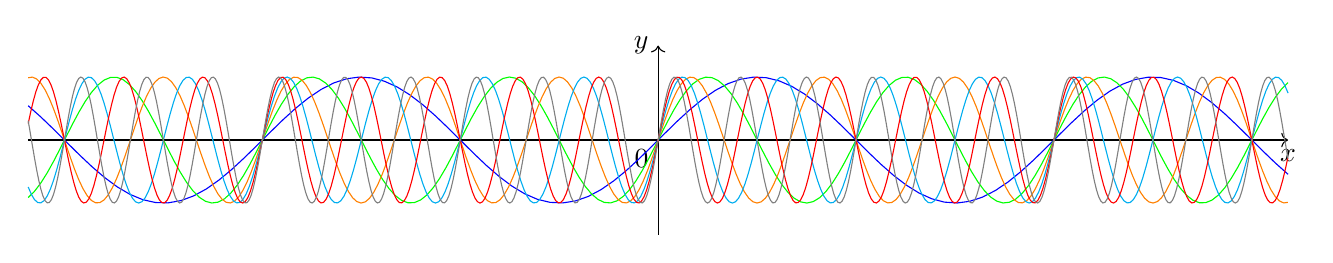
\begin{tikzpicture}[scale=.8]
\draw[->] (-10.,0)--(10.,0) node[below]{$x$};   
\draw[->] (0,-1.5)--(0,1.5)  node[left]{$y$};
\path
(0,0) node[below left]{$0$};
\draw[blue, domain=-10:10, samples=100, variable=\x] plot ({\x}, {(sin ( \x r))});
\draw[green, domain=-10:10, samples=200, variable=\x] plot ({\x}, {(sin ( 2 * \x r))});
\draw[orange, domain=-10:10, samples=300, variable=\x] plot ({\x}, {(sin ( 3 * \x r))});
\draw[cyan, domain=-10:10, samples=400, variable=\x] plot ({\x}, {(sin ( 4 * \x r))});
\draw[red, domain=-10:10, samples=500, variable=\x] plot ({\x}, {(sin ( 5 * \x r))});
\draw[gray, domain=-10:10, samples=600, variable=\x] plot ({\x}, {(sin ( 6 * \x r))});
\end{tikzpicture}
\end{center}
\caption{The sine function.}
\label{fig: 4.3}
\end{figure} \vspace{1 cm}
$$e^{-n \sqrt{x}} \leq 1 \qquad \forall n \in \mathbb{N} \qquad x \geq 1$$
\begin{figure}[!ht]
\begin{center}
\begin{tikzpicture}[scale=6.]
\draw[->] (-0.2,0)--(2.5,0) node[below]{$x$};   
\draw[->] (0,-0.2)--(0,0.5)  node[left]{$y$};
\path
(0,0) node[below left]{$0$};
\path
(0.5,0) node[below left]{$0.5$};
\path
(1.0,0) node[below left]{$1.0$};
\path
(1.5,0) node[below left]{$1.5$};ù
\path
(2.0,0) node[below left]{$2.0$};
\path
(2.5,0) node[below left]{$2.5$};
\foreach \i in {0,0.1, 0.2,...,2.5} \draw (\i,-0.02)--(\i,0.02);
\draw[blue, domain=1:2.5, samples=100, variable=\x] plot ({\x}, {(exp(- sqrt (\x)});
\draw[green, domain=1:2.5, samples=200, variable=\x] plot ({\x}, {(exp(-2 * sqrt (\x)});
\draw[orange, domain=1:2.5, samples=300, variable=\x] plot ({\x}, {(exp(-3 * sqrt (\x)});
\draw[red, domain=1:2.5, samples=400, variable=\x] plot ({\x}, {(exp(-4 * sqrt (\x)});
\end{tikzpicture}
\end{center}
\caption{The sequence of functions $e^{-n \sqrt{x}}$.}
\label{fig: 4.3}
\end{figure}
$$\star \leq |\frac{1}{x^3}| = \frac{1}{x^3} = g(x) \qquad \forall n \in \mathbb{N}$$
since $x \in [0, +\infty)$. Now we need to verify if $g \in L^1([0, +\infty))$. 
$$\int_1^{+\infty} |g(x)| dx = \int_1^{+\infty} |\frac{1}{x^3}| dx = \int_1^{+\infty} \frac{1}{x^3} dx < +\infty$$
since the summability criteria:
$$\int_1^{+\infty} \frac{1}{x^{\alpha}} dx = \begin{cases}
												\frac{1}{\alpha - 1} \qquad if \quad \alpha > 1 \\
												+\infty \qquad if \quad \alpha \leq 1
											\end{cases}$$
Now we can apply the Dominated Convergence Theorem (or Lebesgue Theorem):
$$\lim_{n \rightarrow +\infty} f_n(x) dx = \int_1^{+\infty} \lim_{n \rightarrow +\infty} f_n(x) dx = \int_1^{+\infty} \lim_{n \rightarrow +\infty} \frac{\sin(nx)}{x^3} e^{-n \sqrt{x}} dx = \int_1^{+\infty} 0 dx = 0.$$
Then the solution is
$$\lim_{n \rightarrow + \infty} \int_1^{+\infty} f_n(x) dx = \lim_{n \rightarrow +\infty} \frac{\sin(nx)}{x^3} e^{-n \sqrt{x}} dx = 0 \qquad \forall x \leq 1.$$
\clearpage
\section*{Exercise $2$}
Compute
$$\lim_{n \rightarrow \infty} \int_0^1 f_n(x) dx$$
where 
$$f_n(x) = \frac{x}{1 + x^{2n}} \qquad \textrm{with} \qquad x \in (0, 1).$$
\section*{Solution}
We need to apply the Dominated Converge Theorem. \par 
First of all we analyze the \textbf{pointwise convergence}.
$$\lim_{n \rightarrow \infty} f_n(x) = \lim_{n \rightarrow \infty} \frac{x}{1 + x^{2n}},$$
if $x 	\in [0, 1)$ we have
$$\lim_{n \rightarrow \infty} \frac{x}{1 + x^{2n}} = x$$
since $x^{2n} \rightarrow 0$ for $x \in [0, 1)$. \par
If $x = 1$,
$$\lim_{n \rightarrow \infty} \frac{x}{1 +x^{2n}} = \lim_{n \rightarrow \infty} \frac{1}{1 + 1^{2n}} = \frac{1}{2}.$$
The pointwise limit is
$$\lim_{n \rightarrow \infty} f_n(x) = \begin{cases}
										x \qquad \textrm{if} \qquad x \in [0, 1) \\
										\frac{x}{2} \qquad \textrm{if} \qquad x = 1
									  \end{cases}$$ 
\begin{figure}[!ht]
\begin{center}
\begin{tikzpicture}[scale=5.]
\draw[->] (-1.,0)--(2.,0) node[below]{$x$};   
\draw[->] (0,-0.5)--(0,1.5)  node[left]{$y$};
\draw[dashed] (1,-0.5)--(1,1.5);
\path
(0,0) node[below left]{$0$};
\path
(1,0) node[below left]{$1$};
\foreach \i in {0,0.1, 0.2,...,1.0} \draw (\i,-0.02)--(\i,0.02);
\draw[blue, domain=0:1, samples=100, variable=\x] plot ({\x}, {\x / (1 + \x^2});
\draw[green, domain=0:1, samples=100, variable=\x] plot ({\x}, {\x / (1 + \x^4});
\draw[orange, domain=0:1, samples=100, variable=\x] plot ({\x}, {\x / (1 + \x^6});
\draw[cyan, domain=0:1, samples=100, variable=\x] plot ({\x}, {\x / (1 + \x^8});
\draw[red, domain=0:1, samples=100, variable=\x] plot ({\x}, {\x / (1 + \x^10});
\end{tikzpicture}
\end{center}
\end{figure} \vspace{1 cm}
\begin{figure}[!ht]
\begin{center}
\begin{tikzpicture}[scale=5.]
\draw[->] (-1.,0)--(2.,0) node[below]{$x$};   
\draw[->] (0,-0.5)--(0,1.5)  node[left]{$y$};
\draw[dashed] (1,-0.5)--(1,1.5);
\path
(0,0) node[below left]{$0$};
\path
(1,0) node[below left]{$1$};
\foreach \i in {0,0.1, 0.2,...,1.0} \draw (\i,-0.02)--(\i,0.02);
\draw[blue, domain=0:1, samples=100, variable=\x] plot ({\x}, {\x});
\draw[thick,red, fill=red, opacity=1.0] (1 ,0.5) circle({0.01});  
\end{tikzpicture}
\end{center}
\end{figure} \vspace{1 cm}
Now we find the dominant function.
$$\exists g \in L^1(0, 1) \qquad \textrm{s. t.} \qquad |f_n(x)| \leq g?$$
$$|f_n(x)| = |\frac{x}{1 + x^{2n}}| \leq \frac{x}{1 + x^{2n}} \leq x = g(x) \qquad \forall n \in \mathbb{N}, \qquad \forall x \in (0, 1).$$
$$\int_0^1 |g(x)| dx = \int_0^1 |x| dx = \int_0^1 x dx = [ \frac{x^2}{2}]_0^1 = \frac{1}{2} < +\infty$$
so that
$$g \in L^1(0,1).$$
We can now apply the Dominated Convergence Theorem.
$$\lim_{n \rightarrow \infty} \int_0^1 \frac{x}{1 + x^{2n}} dx = \int_0^1 \lim_{n \rightarrow \infty} \frac{x}{1 + x^{2n}} dx = \int_0^1 x dx = \frac{1}{2}.$$
The solution is
$$\lim_{n \rightarrow \infty} \int_0^1 \frac{x}{1 + x^{2n}} dx = \frac{1}{2}.$$
\clearpage
\section*{Exercise $3$}
Studying convergence in $L^1([1, +\infty))$ of
$$f_n(x) = \frac{\cos(nx)}{n^2 + x} \frac{1}{x^2} \qquad \forall x \geq 1 \qquad \forall n \in \mathbb{N}.$$
\section*{Solution}
\begin{figure}[!ht]
\begin{center}
\begin{tikzpicture}[scale=1.5]
\draw[->] (-0.5,0)--(10.,0) node[below]{$x$};   
\draw[->] (0,-0.5)--(0,1.5)  node[left]{$y$};
\draw[dashed] (1,-0.5)--(1,1.5);
\path
(0,0) node[below left]{$0$};
\path
(1,0) node[below left]{$1$};
\path
(10,0) node[below left]{$10$};
\foreach \i in {1.,1.1, 1.2,...,10.0} \draw (\i,-0.02)--(\i,0.02);
\draw[blue, domain=1.:10., samples=100, variable=\x] plot ({\x}, {(cos(\x) / (1 + \x)) * (1. / \x^2)});
\draw[green, domain=1.:10., samples=100, variable=\x] plot ({\x}, {(cos(2 * \x) / (4. + \x)) * (1. / \x^2)});
\draw[orange, domain=1.:10., samples=100, variable=\x] plot ({\x}, {(cos(3 * \x) / (9. + \x)) * (1. / \x^2)});
\draw[magenta, domain=1.:10., samples=100, variable=\x] plot ({\x}, {(cos(4 * \x) / (16. + \x)) * (1. / \x^2)});
\draw[red, domain=1.:10., samples=100, variable=\x] plot ({\x}, {(cos(5 * \x) / (25. + \x)) * (1. / \x^2)});
\end{tikzpicture}
\end{center}
\end{figure} \vspace{1 cm}
Convergence in $L^1([0, +\infty))$:
$$\norm{f_n - f}_{L^1([1; +\infty))} = \int_1^{+\infty} |f_n - f| dx \rightarrow 0$$
\textbf{POINTWISE CONVERGENCE}
$$\lim_{n \rightarrow \infty} f_n(x) = \lim_{n \rightarrow \infty} \frac{\cos(nx)}{n^2 + x} \frac{1}{x^2} = \star$$
$$-1 \leq \cos(nx) \leq 1$$
$$\star = 0,$$ù
so the pointwise limit is
$$f(x) = 0 \qquad \forall x \geq 1.$$
Now we need to find a dominant function:
$$\exists g \in L^1([1; +\infty)) \qquad \textrm{s.t.} \qquad |f_n(x)| \leq g \qquad \forall x \geq 1 \qquad \forall n \in \mathbb{N}$$
$$|f_n(x)| = |\frac{\cos(nx)}{n^2 + x} \frac{1}{x^2}| \leq \frac{1}{n^2 + x} \frac{1}{x^2} \leq \frac{1}{x} \frac{1}{x^2} =\frac{1}{x^3} = g(x) \qquad \forall x \geq 1 \qquad \forall n \in \mathbb{N}$$
$$\int_1^{+\infty} |g(x)| dx = \int_1^{+\infty} |\frac{1}{x^3}| dx = \int_1^{+\infty} \frac{1}{x^3} dx < +\infty$$
summability criteria:
$$\int_1^{+\infty} \frac{1}{x^{\alpha}} dx = \begin{cases}
												\frac{1}{\alpha - 1} \qquad if \quad \alpha > 1 \\
												+\infty \qquad if \quad \alpha \leq 1,
											\end{cases}$$
then
$$g \in L^1[1; +\infty).$$
$$\lim_{n \rightarrow \infty} \norm{f_n - f}_{L^1([1; +\infty))} \rightarrow 0$$
$$\lim_{n \rightarrow \infty} |f_n - f| dx \rightarrow 0$$
$$iff$$
$$\lim_{n \rightarrow \infty} \int_1^{+\infty} |f_n| dx \rightarrow 0.$$
Now we can apply the Dominated Convergence Theorem:
$$\lim_{n \rightarrow +\infty} \int_1^{+\infty} |f_n| dx = \int_1^{+\infty} \lim_{n \rightarrow +\infty} |f_n| dx = \int_1^{+\infty} \lim_{n \rightarrow +\infty} |\frac{\cos(nx}{n^2 + x} \frac{1}{x^2}| dx$$
$$= \int_1^{+\infty} \lim_{n \rightarrow +\infty} (\frac{\cos(nx)}{n^2 + x} \frac{1}{x^2} dx = \int_1^{+\infty} 0 dx = 0,$$
so that
$$f_n \rightarrow 0 \qquad \textrm{in} \qquad L^1([1; +\infty)).$$									
\clearpage
\section*{Exercise $4$}
Let $f_n(x) = \sum_{n=1}^{\infty} \frac{|\sin(nx)|}{2^n} \qquad x \in [0, \pi]$. Compute
$$\int_0^{\pi} f(x) dx.$$
\section*{Solution}
Remember that a series is the limit of the partial sums. If the partial sums are formed by positive terms, then the series are monotone. We consider
$$f_h(x) = \sum_{n = 1}^{h} \frac{|\sin(nx)|}{2^n}.$$
We have truncated the series up to the $h$ term. If we consider the truncated series we have that $f_h(x)$ is monotone, in fact
$$0 \leq f_h \leq f_{h + 1}.$$
Furthermore 
$$f_h(x) = \sum_{h=1}^{h} \frac{|\sin(nx)|}{2^n} \rightarrow f(x) \qquad \textrm{for} \qquad h \rightarrow \infty.$$
Then we can apply the Beppo Levi's Theorem:
$$\int_0^{\pi} f(x) dx = \int_0^{\pi} \lim_{h \rightarrow \infty} f_h(x) dx = \lim_{h \rightarrow \infty} \int_0^{\pi} f_h(x) dx = \lim_{h \rightarrow \infty} \int_0^{\pi} \sum_{n=1}^{h} \frac{|\sin(nx)|}{2^n} dx = \lim_{h \rightarrow \infty} \sum_{n=1}^h \frac{1}{2^n} \int_0^{\pi} |\sin(nx)| dx.$$
Now we have to compute the integral. We know that
$$\int_0^{\infty} |\sin(y)| dy = n \int_0^{\pi} \sin(y) dy$$
so that
$$\int_0^{\pi} |\sin(nx)| dx = \int_0^{n \pi} |sin y| \frac{dy}{n} = \int_0^{\pi} \sin y dy = [-\cos y]_0^{\pi} = 2.$$
Then
$$\int_0^{\pi} f(x) dx = \sum_{k=1}^{\infty} (\frac{1}{2})^k 2 = \sum_{k=1}^{\infty} \frac{2}{2^k} = 2.$$
Then
$$\int_0^{\pi} f(x) dx = 2.$$ 
\clearpage
\section*{Exercise $5$}
Compute
$$\int_0^{+\infty} \frac{1}{\sqrt{x}} \sum_{k = 0}^{\infty} e^{-(\alpha^n)\sqrt{x}} dx$$
as $\alpha \geq 0$ varies.
\section*{Solution}
Consider
$$\sum_{k = 0}^{\infty} e^{l(\alpha)^k \sqrt{x}},$$
it is a series with positive terms, then it converges or positively diverges, that is well defined. If we consider its truncated
$$\sum_{k = 0}^n e^{-(\alpha^k) \sqrt{x}}$$
we can construct the functions
$$f_{\alpha, n} (x) = \sum_{k = 0}^n e^{-(\alpha^k)\sqrt{x}}.$$
This is a sequence of functions $f_n \geq 0$ with
$$0 \leq f_n \leq f_{n+1} \qquad \forall n \in \mathbb{N},$$
then it is monotone. We can use the Beppo Levi Theorem:
$$\int_0^{+infty} \frac{1}{\sqrt{x}} \sum_{k = 0}^{+\infty} e^{-(\alpha^k)\sqrt{x}} dx = \int_0^{+\infty} \frac{1}{\sqrt{x}} \lim_{n \rightarrow \infty} \sum_{k = 0}^n e^{-(\alpha^k)\sqrt{x}} dx = \star$$
now we can apply Beppo Levi Theorem
$$\star = \lim_{n \rightarrow \infty} \sum_{k = 0}^n \int_0^{+\infty} \frac{e^{-(\alpha^k)\sqrt{x}}}{\sqrt{x}} dx = \star$$
now we can make a change of variables,
$$y = \sqrt{x}$$
$$dy = \frac{1}{2} \frac{1}{y} dx$$
$$dx = 2 y dy$$
$$\star = \lim_{n \rightarrow \infty} \sum_{k = 0}^n \int_0^{\infty} \frac{e^{-(\alpha^k) y}}{y} 2 y dy = \lim_{n \rightarrow \infty} \sum_{k = 0}^{\infty} 2 \int_0^{\infty} e^{-(\alpha^k) y} dy$$
Now we have that
$$[e^{-(\alpha^k)y}]' = -(\alpha^k) e^{-(\alpha^k)y}$$
then
$$\lim_{n \rightarrow \infty} \sum_{k = 0}^n 2 \frac{1}{(-\alpha^k)} \int_0^{\infty} -(\alpha^k)e^{-(\alpha^k)y} dy = \lim_{n \rightarrow \infty} \sum_{k=0}^n 2 \frac{1}{-(\alpha^k)}\int_0^{\infty} [e^{-(\alpha^k)y}]'$$
$$ = \sum_{k = 0}^{+\infty} \frac{2}{-\alpha^k} (\lim_{c \rightarrow \infty} [e^{-(\alpha^k)y}]_0^c) = \sum_{k=0}^{\infty} \frac{2}{\alpha^k} = 2 \sum_{k=0}^{\infty}(\frac{1}{\alpha})^k= \star$$
this is a geometric series, then
$$\star = 2 \begin{cases}
				+\infty \qquad \textrm{if} \qquad \frac{1}{\alpha} \geq 1 \\
				\frac{1}{1 - \frac{1}{\alpha}} \qquad \textrm{if} \qquad |\frac{1}{\alpha}| < 1 \\
				\textrm{indet.} \qquad \textrm{if} \qquad \frac{1}{\alpha} \leq -1.
			\end{cases}$$
But we have that $\alpha \geq 0$, then
$$\int_0^{\infty} \frac{1}{\sqrt{x}} \sum_{k=0}^{\infty} e^{-(\alpha^k)\sqrt{x}} dx = \begin{cases}
		\frac{2 \alpha}{\alpha - 1} \qquad \textrm{if} \qquad \frac{1}{\alpha} \in (0, 1) \\
		\infty \qquad \textrm{if} \qquad \frac{1}{\alpha} \geq 1	 
	 \end{cases} = \begin{cases}
		\frac{2 \alpha}{\alpha - 1} \qquad \textrm{if} \qquad \alpha > 1 \\
		\infty \qquad \textrm{if} \qquad \alpha \in (0, 1].	 
	 \end{cases}$$
\clearpage
\section*{Exercise $6$}
Let $g \in L^p(\R)$, $1 \leq p \leq +\infty$. Studying the convergence in $L^p$ of
$$f_n(x) = \arctan{(n |x|)} \cdot g(x) \qquad \forall x \in \R, \qquad n \in \N$$
\section*{Solution}
$$f_n(x) = \arctan(n |x|) \cdot g(x) \qquad \forall x \in \R, \qquad n \in \N$$
First of all we need to know the pointwise limit of the function. We can consider
$$\phi_n(x) = \arctan(n |x|) \qquad \forall x \in \R, \qquad n \in \N$$
\begin{figure}[!ht]
\begin{center}
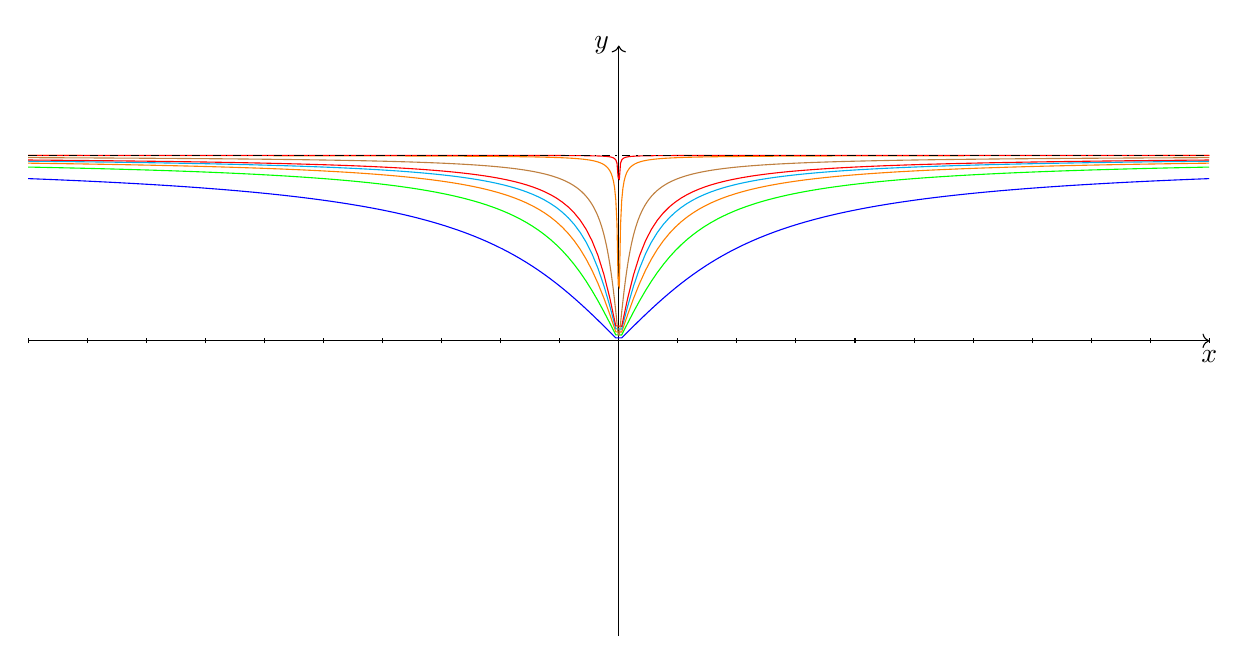
\begin{tikzpicture}[scale=1.5, trig format=rad]
\draw[->] (-5.,0)--(5.,0) node[below]{$x$};   
\draw[->] (0,-2.5)--(0,2.5)  node[left]{$y$};
\foreach \i in {-5.,-4.5,-4.,...,0., ..., 4., 4.5,5.0} \draw (\i,-0.02)--(\i,0.02);
\draw[blue, domain=-5.:5., samples=200, variable=\x] plot ({\x}, {atan(abs(\x))});
\draw[green, domain=-5.:5., samples=200, variable=\x] plot ({\x}, {atan(2*abs(\x))});
\draw[orange, domain=-5.:5., samples=200, variable=\x] plot ({\x}, {atan(3*abs(\x))});
\draw[cyan, domain=-5.:5., samples=200, variable=\x] plot ({\x}, {atan(4*abs(\x))});
\draw[red, domain=-5.:5., samples=200, variable=\x] plot ({\x}, {atan(5*abs(\x))});
\draw[brown, domain=-5.:5., samples=1000, variable=\x] plot ({\x}, {atan(10*abs(\x))});
\draw[orange, domain=-5.:5., samples=1000, variable=\x] plot ({\x}, {atan(100*abs(\x))});
\draw[red, domain=-5.:5., samples=1000, variable=\x] plot ({\x}, {atan(1000*abs(\x))});
\draw[dash dot, domain=-5.:5., samples=100, variable=\x] plot ({\x}, {pi/2.});
\end{tikzpicture}
\end{center}
\end{figure} \vspace{1 cm}
The pointwise limit of the function is:
$$
\lim_{n \rightarrow +\infty} \phi_n(x) = 
\begin{cases}
0 \qquad \textrm{if} \qquad x = 0 \\
\frac{\pi}{2} \qquad \textrm{if} \qquad x \neq 0
\end{cases}.$$
So that from the measure theory we have:
$$\phi_n \rightarrow \frac{\pi}{2} \qquad \mu - q.o. \qquad \textrm{in} \qquad \R$$
The function $g$ doesn't depend on $n$, then:
$$\lim_{n \rightarrow +\infty} f_n(x) = \lim_{n \rightarrow + \infty} \phi_n \cdot g = \frac{\pi}{2} \cdot g \qquad \mu-q.o. \qquad \textrm{in} \qquad \R.$$
The pointwise limit of the functions $f_n(x)$ is $\frac{\pi}{2} \cdot g.$ \par 
From the definition of the convergence in the $L^p$ spaces we need 
$$\norm{f_n - f}_{L^p} = ?$$
where $f$ is the pointwise limit. We need to use the Dominated Convergence Theorem. \par 
Now we search for the domination function.
$$\norm{f_n - f}_{L^p(\R)} = \int_{\R} |f_n - f|^p dx = \star$$
$$|f_n(x) - \frac{\pi}{2}g(x)| = |\arctan(n|x|) \cdot g(x) - \frac{\pi}{2} g(x)|$$
$$-\frac{\pi}{2} \leq \arctan{(n|x|)} \leq \frac{\pi}{2}$$
$$\star = |g(x)| |\arctan{(n|x|)} - \frac{\pi}{2}|$$
then
$$|f_n(x) - \frac{\pi}{2} g(x)|^p = |g(x)|^p |\arctan{(n|x|)} - \frac{\pi}{2}|^p \leq (\frac{\pi}{2})^p |g(x)|^p$$
for $\mu-q.o. \qquad x \in \R \qquad \textrm{and} \qquad \forall n \in \N$. \par
\vspace{0.5 cm}    
By hypotheses $g \in L^p(\R)$, then $|g|^p \in L^1(\R)$ and so $(\frac{\pi}{2})^p |g(x)|^p \in L^1(\R)$. \par 
\vspace{0.5 cm}
We can apply the Dominated Convergence Theorem.
$$\lim_{n \rightarrow +\infty} \norm{f_n - f}_{L^p(\R}^p = \lim_{n \rightarrow +\infty} \int_{\R} |f_n(x) - f(x)|^p dx = \int_{\R} \lim_{n \rightarrow +\infty} |f_n(x) - f(x)|^p dx = $$
$$= \int_{\R} \lim_{n \rightarrow +\infty} |\arctan{(n |x|)} \cdot g(x) - \frac{\pi}{2} g(x)|^p dx \leq |g(x)|^p \int_{\R} \int_{\R} \lim_{n \rightarrow +\infty} |\arctan{(n |x|)} - \frac{\pi}{2}|^p dx = $$
$$= |g(x)|^p \int_{\R} |\frac{\pi}{2} - \frac{\pi}{2}| dx = 0$$
then
$$\lim_{n \rightarrow +\infty} \norm{f_n - f}_{L^p(\R)} \rightarrow 0$$
$$\iff$$
$$f_n \rightarrow f \qquad \textrm{in} \qquad L^p(\R)$$
for $n \rightarrow +\infty$. Then
$$f_n(x) \rightarrow \frac{\pi}{2} g(x) \qquad \mu-q.o. \qquad \forall x \in \R \qquad \textrm{in} \qquad L^p(\R) \qquad \textrm{for} \qquad n \rightarrow +\infty .$$
\clearpage
\section*{Exercise $7$}
Let 
$$f_n(x) := \frac{\sin(nx)}{n^2 x^{\frac{3}{2}}} \qquad \forall x \in (0, +\infty), \qquad \forall n \in \N.$$
Compute the limit of $\{ f_n \} \qquad \textrm{in} \qquad L^1((0, + \infty))$. 
\section*{Solution}
Let draw the graph of $f_n(x)$.
\begin{figure}[!ht]
\begin{center}
\begin{tikzpicture}[scale=1.0, trig format=rad]
\draw[->] (0.,0)--(10.,0) node[below]{$x$};   
\draw[->] (0,-0.5)--(0,12.0)  node[left]{$y$};
\foreach \i in {0.,0.5, 1.0,  ..., 4., 4.5,5.0, ..., 8.0, 8.5, 9.0, 9.5, 10.0} \draw (\i,-0.02)--(\i,0.02);
\draw[blue, domain=0.01:10., samples=200, variable=\x] plot ({\x}, {sin(\x)/(\x^(3/2))});
\draw[cyan, domain=0.01:10., samples=200, variable=\x] plot ({\x}, {sin(2*\x)/(2^2*\x^(3/2))});
\draw[green, domain=0.01:10., samples=200, variable=\x] plot ({\x}, {sin(3*\x)/(3^2*\x^(3/2))});
\draw[orange, domain=0.01:10., samples=200, variable=\x] plot ({\x}, {sin(4*\x)/(4^2*\x^(3/2))});
\draw[magenta, domain=0.01:10., samples=200, variable=\x] plot ({\x}, {sin(5*\x)/(5^2*\x^(3/2))});
\draw[red, domain=0.01:10., samples=200, variable=\x] plot ({\x}, {sin(6*\x)/(6^2*\x^(3/2))});
\end{tikzpicture}
\end{center}
\end{figure} \vspace{1 cm}
We have
$$f_n(x) \sim \frac{\bcancel{n} x}{n^{\bcancel{2} x^{\frac{3}{2}}}} = \frac{1}{n \sqrt{x}} \qquad \textrm{for} \qquad x \rightarrow 0^+, \qquad \forall n \in \N,$$
furthermore
$$|f_n(x)| \leq \frac{1}{n^2 x^{\frac{3}{2}}} \qquad \forall x \in (0, +\infty) \qquad \forall n \in \N^+.$$
If we consider the summability criteria
$$\int_1^{+\infty} \frac{1}{x^{\alpha}} dx = \begin{cases}
												\frac{1}{\alpha - 1} \qquad \textrm{if} \qquad \alpha > 1\\
												+\infty \qquad \textrm{if} \qquad \alpha \leq 1
											\end{cases}$$
$$\int_0^1 \frac{1}{x^{\alpha}} dx = \begin{cases}
												\frac{1}{\alpha - 1} \qquad \textrm{if} \qquad \alpha < 1\\
												+\infty \qquad \textrm{if} \qquad \alpha \geq 1
											\end{cases}$$
we have that
$$\{ f_n \} \subset L^1((0, +\infty))$$
\vspace{0.5 cm}
\textbf{POINTWISE CONVERGENCE}
\vspace{0.5 cm}
$$\lim_{n \rightarrow + \infty} f_n(x) = \lim_{n \rightarrow +\infty} \frac{\sin(n x)}{n^2 x^{\frac{3}{2}}} = \lim_{n \rightarrow +\infty} \frac{\sin (n x)}{n x} \frac{1}{n \sqrt{x}} =$$
$$= \lim_{n \rightarrow + \infty} \frac{\sin (n x)}{x^{\frac{3}{2}}}  \cdot \frac{1}{n^2} = \textrm{\textbf{bounded}} \cdot 0 = 0$$
So that 
$$f(x) = 0 \qquad \textrm{is the pointwise limit} \qquad \forall x \in (0, +\infty),$$
hence
$$f_n \rightarrow 0 \qquad \textrm{for} \qquad n \rightarrow +\infty \qquad \textrm{in} \qquad (0, +\infty).$$
Now we search for the dominant function. We have that $\forall x \in (0, +\infty) \qquad \textrm{and} \qquad n \in \N^+$,
$$|f_n(x)| \leq \phi(x) := \begin{cases}
							\frac{1}{\sqrt{x}} \qquad x \in (0, 1] \\
							\frac{1}{x^{\frac{3}{2}}} \qquad x > 1
						  \end{cases}$$
For the summability criteria we have that 
$$\phi \in L^1((0, +\infty)).$$
Now we can apply the Dominated Convergence Theorem:
$$\lim_{n \rightarrow +\infty} \norm{f_n - 0}_{L^1((0, +\infty))} = \lim_{n \rightarrow +\infty} \int_0^{+\infty} f_n(x) dx = \lim_{n \rightarrow + \infty} \int_0^{+\infty} \frac{\sin(n x)}{n^2 x^{\frac{3}{2}}} dx $$
$$= \int_0^{+\infty} \lim_{n \rightarrow +\infty} \frac{\sin(n x)}{n^2 x^{\frac{3}{2}}} dx = 0$$
$$f_n \rightarrow 0 \qquad \textrm{for} \qquad n \rightarrow +\infty \qquad \textrm{in} L^1((0, +\infty)).$$
So the limit of $\{ f_n \}$ in $L^1((0, +\infty))$ is zero.
\clearpage
\chapter{$L^p$ Spaces}
\section*{Exercise $1$}
Analyze the convergence in $L^p([0, 1])$ with $1 \leq p < \infty$ of
$$f_n(x) = \frac{\cos(nx) e^{-n x}}{\sqrt[4]{x}} \qquad for \quad x \in [0, 1] \qquad \forall n \in \mathbb{N}.$$
For which $L^p$ the sequence converge to a certain function?
\section*{Solution}
\begin{figure}[!ht]
\begin{center}
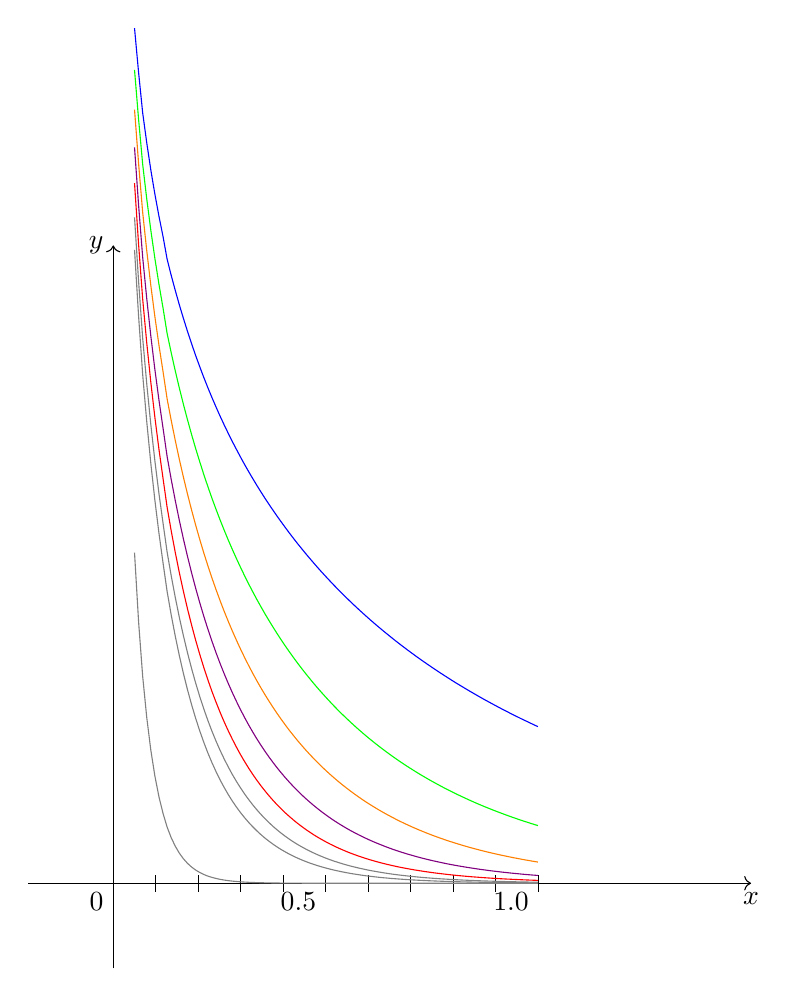
\begin{tikzpicture}[scale=5.4]
\draw[->] (-0.2,0)--(1.5,0) node[below]{$x$};   
\draw[->] (0,-0.2)--(0,1.5)  node[left]{$y$};
\path
(0,0) node[below left]{$0$};
\path
(0.5,0) node[below left]{$0.5$};
\path
(1.0,0) node[below left]{$1.0$};
\foreach \i in {0,0.1, 0.2,...,1.0} \draw (\i,-0.02)--(\i,0.02);
\draw[blue, domain=0.05:1.0, samples=100, variable=\x] plot ({\x}, {(cos (\x) / \x^(1 / 4) * exp(- \x)});
\draw[green, domain=0.05:1.0, samples=100, variable=\x] plot ({\x}, {(cos (2 * \x) / \x^(1 / 4) * exp(-2* \x)});
\draw[orange, domain=0.05:1.0, samples=100, variable=\x] plot ({\x}, {(cos (3 * \x) / \x^(1 / 4) * exp(- 3 * \x)});
\draw[violet, domain=0.05:1.0, samples=100, variable=\x] plot ({\x}, {(cos (4 * \x) / \x^(1 / 4) * exp(-4* \x)});
\draw[red, domain=0.05:1.0, samples=100, variable=\x] plot ({\x}, {(cos (5 * \x) / \x^(1 / 4) * exp(-5* \x)});
\draw[gray, domain=0.05:1.0, samples=100, variable=\x] plot ({\x}, {(cos (6 * \x) / \x^(1 / 4) * exp(-6* \x)});
\draw[gray, domain=0.05:1.0, samples=100, variable=\x] plot ({\x}, {(cos (7 * \x) / \x^(1 / 4) * exp(-7* \x)});
\draw[gray, domain=0.05:1.0, samples=100, variable=\x] plot ({\x}, {(cos (20 * \x) / \x^(1 / 4) * exp(-20* \x)});
\end{tikzpicture}
\end{center}
\caption{The sequence of functions $f_n(x)$.}
\label{fig: 4.3}
\end{figure}
First of all we search for which $p$ this sequence belongs to some $L^p$, applying the Dominated Convergence Theorem.
$$|f_n(x)| = |\frac{\cos(nx)}{\sqrt[4]{x}} e^{-n x}| \leq \frac{1}{\sqrt[4]{x}} = g(x) \qquad x \in [0, 1]$$
We know that $f_n(x)$ belongs to some $L^p$ if and only if
$$\int_0^1 |f_n(x)|^p dx < +\infty.$$
The exponents $p$ that satisfy this relations are the candidates.
$$\int_0^1 |f_n(x)|^p dx = \int_0^1 |\frac{\cos(nx)}{\sqrt[4]{x}} e^{-n x}|^p dx \leq \int_0^1 |\frac{1}{\sqrt[4]{x}}|^p dx = \int_0^1 \frac{1}{x^{\frac{p}{4}}} dx.$$
From the summability criteria:
$$\int_1^{+\infty} \frac{1}{x^{\alpha}} dx = \begin{cases}
												\frac{1}{\alpha - 1} \qquad if \quad \alpha > 1 \\
												+\infty \qquad if \quad \alpha \leq 1
											\end{cases},$$
since
$$|\frac{\cos(nx)}{\sqrt[4]{x}} e^{-n x}|^p \leq \bigl( \frac{1}{\sqrt[4]{x}} \bigl)^p$$
we have that for $p \in [1, 4) \qquad f_n(x) \in L^p([0, 1]) \qquad \forall n \in \mathbb{N}.$
\begin{itemize}
\item $f_n \in L^1([0, 1])$;
\item $f_n \in L^2([0, 1])$;
\item $f_n \in L^3([0, 1])$.
\end{itemize}
\textbf{Pointwise Convergence}:
$$\lim_{n \rightarrow +\infty} f_n(x) = \lim_{n \rightarrow +\infty} \frac{\cos(nx)}{\sqrt[4]{x}} e^{-nx} = \lim_{n \rightarrow +\infty} \frac{\cos(nx)}{\sqrt[4]{x} e^{nx}} \rightarrow 0$$
so
$$f_n \rightarrow 0 \qquad \textrm{pointwise} \qquad \forall x \in [0,1],$$
we can apply the comparison criterium.
$$\lim_{x \rightarrow 0^+} f_n(x) \sqrt[4]{x} = \lim_{x \rightarrow 0^+} \frac{\cos(nx)}{\sqrt[4]{x}}e^{-nx} \sqrt[4]{x} = 1$$
$$f_n(x) \sim \frac{1}{\sqrt[4]{x}} \qquad \textrm{for} \qquad x \rightarrow 0^+.$$
Now we can analyze the convergence in $L^p([0, 1])$
$$\norm{f_n - f}_{L^p}$$
$$\norm{f_n(x) - f(x)}_{L^p([0, 1])}^p = \norm{f_n(x)}_{L^p([0,1])}^p = \norm{\frac{\cos(nx)}{\sqrt[4]{x} e^{nx}}}_{L^p([0,1])}^p = \int_0^1 |\frac{\cos(nx)}{\sqrt[4]{x} e^{-nx}}_{L^p([0,1])}|^p dx = \star$$
since
$$|\frac{\cos(nx)}{\sqrt[4]{x} e^{nx}}_{L^p([0,1])}|^p \leq g(x) = \frac{1}{x^{\frac{p}{4}}}$$
where
$$g \in L^p([0,1]) \qquad \textrm{for} \qquad 1 \leq p < 4,$$
we can apply the Dominated Convergence Theorem
$$\lim_{n \rightarrow +\infty} \norm{f_n(x) - f(x)}_{L^p([0, 1])}^p = \lim_{n \rightarrow +\infty} \int_0^1 |\frac{\cos(nx)}{\sqrt[4]{x}}e^{-nx}|^p dx = \int_0^1 \lim_{n \rightarrow +\infty} |\frac{\cos(nx)}{\sqrt[4]{x}} e^{-nx}|^p dx = 0.$$	
So
$$\lim_{n \rightarrow +infty} \norm{f_n(x) - f(x)}_{L^p([0, 1])} \rightarrow 0$$
$$f_n(x) \rightarrow 0 \qquad in \qquad L^p([0, 1]) \qquad \forall p \in [1; 4).$$
Since
$$\lim_{x \rightarrow 0^+} \frac{|f_n(x)|}{g(x)} = 1 \qquad \forall n \in \mathbb{N}$$
we have
$$f_n \in L^p([0, 1]) \leftrightarrow g \in L^p([0, 1])$$
so that
$$f_n \notin L^p([0, 1]) \qquad \textrm{if} \qquad p \geq 4.$$
The sequence $\{ f_n(x) \}_{n \in \mathbb{N}}$ can't converge in $L^p([0, 1])$ spaces if $p \geq 4$. \par 
In the case $p = +\infty$, we have
$$\norm{f_n(x)}_{\infty} = \esssup_{x \in (0, 1)} |\frac{\cos(nx)}{\sqrt[4]{x}}e^{-nx}| \leq \sup_{x \in (0,1)} |\frac{1}{\sqrt[4]{x}}| \rightarrow +\infty,$$
so
$$f_n \nrightarrow 0 \qquad \textrm{in} \qquad L^{\infty}((0, 1)).$$		
Since $[0, 1]$ is a bounded set we have the following embeddings:	
\begin{figure}[!ht]
\begin{center}
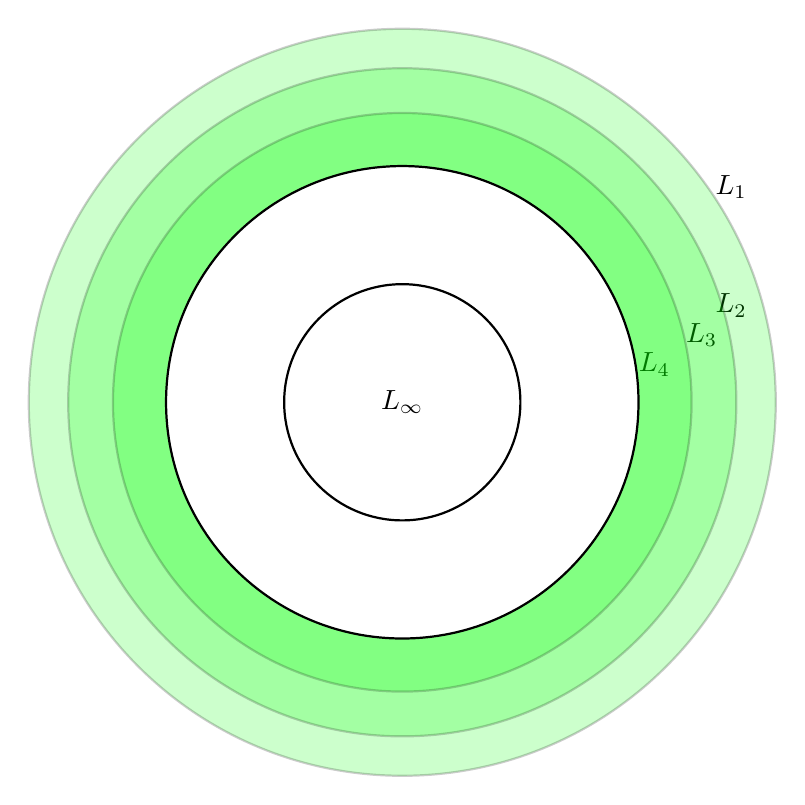
\begin{tikzpicture}[scale=1.5]
\path
(3,2) node[below left]{$\huge{L_1}$};
\path
(3.0,1) node[below left]{$\huge{L_2}$};
\path
(2.75,0.75) node[below left]{$\huge{L_3}$};
\path
(2.35,0.5) node[below left]{$\huge{L_4}$};
\path
(0.5,0.2) node[below left]{$\huge{L_{\infty}}$};
\draw[thick,black, fill=green, opacity=0.2] (0 ,0) circle({sqrt(10)});     
\draw[thick,black, fill=green, opacity=0.2] (0 ,0) circle({sqrt(8)});     
\draw[thick,black, fill=green, opacity=0.2] (0 ,0) circle({sqrt(6)});     
\draw[thick,black, fill=white, opacity=1.0] (0 ,0) circle({sqrt(4)});         
\draw[thick,black, fill=white, opacity=1.0] (0 ,0) circle({sqrt(1)}) node[text=black]{$\huge{L_{\infty}}$};;     
\end{tikzpicture}
\end{center}
\end{figure}							
The sequence $f_n(x)$ lives in "green" spaces.
\clearpage
\section*{Exercise $2$}
Let $f \in L^{\infty}([0, +\infty))$ and suppose it is a monotone non-increasing function (weakly decreasing). Let $f \geq 0$.Show that
$$x = f(x) \rightarrow 0 \qquad \textrm{for} \qquad x \rightarrow + \infty.$$
\section*{Solution}
$f$ is weakly decreasing or monotone non-increasing and it is positive. Then
$$\forall x_1 \leq x_2 \implies f(x_2) \leq f(x_1),$$
furthemore it is positive, then
$$\lim_{x \rightarrow +\infty} f(x) = l$$
that is
$$\lim_{x \rightarrow +\infty} f(x) = l = \inf \{ f(x) \qquad \textrm{s.t.} \qquad x \in dom f, \qquad x > l \}$$
$$f \in L^1([0, +\infty)) \implies l = 0$$
$f \in L^1([0, +\infty))$ means that $\int_0^{+\infty} |f| dx < +\infty$. If it were $l \neq 0$  we would have
$$f \neq L^1([0, +\infty))$$
since
$$\int_0^{+\infty} |f| dx \rightarrow +\infty.$$
If $f \in L^1([0, +\infty))$ it must be $l = 0$. We now need to show that the product $x \cdot f(x) \rightarrow 0$ for $x \rightarrow + \infty$. We have
$$\int_0^{+\infty} f(t) dt = \int_0^{+\infty} f(t) \chi_{[t > x]} dt$$
We have that for $x \rightarrow +\infty \implies \chi_{[t > x]} \rightarrow 0$, in fact:
\begin{figure}[!ht]
\begin{center}
\begin{tikzpicture}[scale=2.5]
\draw[->] (-2.0,0)--(3.5,0) node[below]{$x$};   
\draw[->] (0,-0.5)--(0,2.5)  node[left]{$y$};
\draw[dashed] (1.5,0.0)--(1.5,1.0);
\path
(0,0) node[below left]{$0$};
\path
(0.5,0) node[below left]{$0.5$};
\path
(1.5,0) node[below left]{$x$};
\path
(2.5,1.5) node[below left]{$\chi_{[t > x]}$};
\draw[blue, line width = 1.5, domain=-2.:1.5, samples=100, variable=\x] plot ({\x}, {0});
\draw[blue, line width = 1.5, domain=1.5:3.5, samples=100, variable=\x] plot ({\x}, {1});
\end{tikzpicture}
\end{center}
\end{figure}
for $x \rightarrow + \infty$ it becomes
\begin{figure}[!ht]
\begin{center}
\begin{tikzpicture}[scale=2.5]
\draw[->] (-2.0,0)--(3.5,0) node[below]{$x$};   
\draw[->] (0,-0.5)--(0,2.5)  node[left]{$y$};
\path
(0,0) node[below left]{$0$};
\path
(0.5,0) node[below left]{$0.5$};
\path
(1.5,0) node[below left]{$x$};
\path
(2.5,1.5) node[below left]{$\chi_{[t > x]}$};
\draw[blue, line width = 1.5, domain=-2.:3.5, samples=100, variable=\x] plot ({\x}, {0});
\end{tikzpicture}
\end{center}
\end{figure}
Now we search the domination for $f(t) \chi_{[t > x]}(t)$, beacouse we want to apply the Dominated Convergence Theorem.
$$f(t) \chi_{[t > x]} \leq |f(t)| \qquad \textrm{with} \qquad f \in L^1([0, +\infty))$$
$$\textrm{for} \qquad x \rightarrow +\infty \qquad \textrm{we have}$$
$$f(t) \chi_{[t > x]} \rightarrow 0 \qquad \textrm{a.e.} \mu$$
This function is dominate by $|f(t)|$ that is a $L^1$ function. Then we can apply the Dominated Convergence Theorem.
$$\lim_{t \rightarrow +\infty} \int_0^{+\infty} f(t) dt = \int_0^{+\infty} \lim_{t \rightarrow +\infty} f(t) dt = 0$$
$$\forall \epsilon > 0 \qquad \exists x_{\epsilon} > 0 \qquad \textrm{s.t.} \qquad \int_{x_{\epsilon}}^{+\infty} f(x) < \epsilon.$$
Now we take $x \geq x_{\epsilon}$, we have
$$x f(x) = x_{\epsilon} f(x) + x f(x) - x_{\epsilon} f(x) = x_{\epsilon} f(x) + f(x) \int_{x_{\epsilon}}^x 1 dt \leq \star$$
since it is weakly decreasing we can put $f$ inside the integral
$$\star \leq x_{\epsilon} f(x) + \int_{x_{\epsilon}}^x f(t) dt \leq \star$$
since $f$ is positive then we can integrate between $x_{\epsilon}$ and $+\infty$
$$\star \leq x_{\epsilon} f(x) + \int_{x_{\epsilon}}^{+\infty} f(t) dt.$$
Now we can pass to the limit for $x \rightarrow +\infty$ and we obtain
$$x f(x) \leq x_{\epsilon} f(x) + \int_{x_{\epsilon}}^{+\infty} f(t) dt \leq \epsilon$$
$$\textrm{for} \qquad x \rightarrow +\infty \qquad xf(x) \leq \epsilon \qquad \forall \epsilon >0$$
then for $x \rightarrow +\infty$, $xf(x) \rightarrow 0$.
\clearpage
\section*{Exercise $3$}
Find $f \in (L^1(\mathbb{R}) \cap L_{loc}^{\infty}(\mathbb{R}) \setminus L^2(\mathbb{R})$ and $g \in (L^2(\mathbb{R}) \cap L^{\infty}(\mathbb{R})) \setminus L^1(\mathbb{R})$.
\section*{Solution}
We want to find a function $f$  that belongs to $(L^1(\mathbb{R}) \cap L_{loc}^{\infty}(\mathbb{R}) \setminus L^2(\mathbb{R})$. \par  
First of all we can construct a function that is in $L^1(\mathbb{R})$ and that is locally bounded (essentially bounded), but that is not in $L^2(\mathbb{R})$. \par 
Generally when think to the term "local" we mean "restricted to a compact set". \par 
We can think to the following function:
$$f(x) = \sum_{k = 1}^{\infty} k \chi_{[k, k + \frac{1}{k^3}]} (x) \qquad x \in \mathbb{R}$$
\begin{figure}[!ht]
\begin{center}
\begin{tikzpicture}[scale=2.5]
\draw[->] (-2.0,0)--(3.5,0) node[below]{$x$};   
\draw[->] (0,-0.5)--(0,3.5)  node[left]{$y$};
\draw[dashed] (1.,0.0)--(1.,1.0);
\draw[dashed] (2.,0.0)--(2.,2.0);
\draw[dashed] (17.0/8,0.0)--(17.0/8,2.0);
\draw[dashed] (3.,0.0)--(3.,3.0);
\draw[dashed] (83./27,0.0)--(83./27,3.0);
\path
(0,0) node[below left]{$0$};
\path
(0.5,0) node[below left]{$0.5$};
\path
(1.0,0) node[below left]{$1.0$};
\path
(2.0,0) node[below left]{$2.0$};
\path
(3.0,0) node[below left]{$3.0$};
\path
(0,1.0) node[below left]{$1.0$};
\path
(0.0,2.0) node[below left]{$2.0$};
\path
(0.0,3.0) node[below left]{$3.0$};
\path
(2.0,2.5) node[below left]{$f(x)$};
\foreach \i in {0,1.0, 2.0,...,3.0} \draw (\i,-0.02)--(\i,0.02);
\foreach \i in {0,1.0, 2.0,...,3.0} \draw (-0.02,\i)--(0.02,\i);
\draw[blue, line width = 1.5, domain=-2.:1.0, samples=100, variable=\x] plot ({\x}, {0});
\draw[blue, line width = 1.5, domain=1.0:2.0, samples=100, variable=\x] plot ({\x}, {1});
\draw[blue, line width = 1.5, domain=2.0:17.0/8, samples=100, variable=\x] plot ({\x}, {2});
\draw[blue, line width = 1.5, domain=17.0/8:3, samples=100, variable=\x] plot ({\x}, {0});
\draw[blue, line width = 1.5, domain=3.0:83./27, samples=100, variable=\x] plot ({\x}, {3});
\end{tikzpicture}
\end{center}
\end{figure}
$$f(x) = \chi_{[1, 2]} + 2 \chi_{[2, \frac{17}{8}]} + 3 \chi_{[3,\frac{82}{27}]} + \cdots$$
This function is surely in $L_{loc}^{\infty}(\mathbb{R})$. In fact $\forall a > 0 \exists k_a$ maximal such that $k_a \leq a$. Then
$$f \in L_{loc}^{\infty}.$$
\vspace{1.5 cm}
We know that
$$\sup_{a \in A} f = k_a,$$
since the  rung at the $k$-th step is $k$ high. The norm $L^1$ is given by the sum of the area of each rectangle. Then
$$\norm{f}_{L^1(\mathbb{R})} = \int_{\mathbb{R}} |f| dx < +\infty,$$
$$\frac{1}{k^3} \rightarrow 0 \qquad \textrm{for} \qquad k \rightarrow +\infty.$$
\vspace{1.5 cm}
Now we want to show that $f \notin L^2(\mathbb{R})$. We consider the truncated
$$f_n = \sum_{k = 1}^n k \chi_{k, k + \frac{1}{k^3}} (x),$$
and make all the calculus. Trivially $f_n \geq 0$, then we have a series with positive terms. Furthermore $f_n$ is monotone since
$$0 \leq f_n \leq f_{n + 1}.$$
We can apply the Beppo Levi Theorem (or the Monotone Convergence Theorem).
$$\norm{f}_{L^1(\mathbb{R})} = \int_{\mathbb{R}} |f| dx = \int_{\mathbb{R}} \lim_{n \rightarrow +\infty} \sum_{k = 1}^n k \chi_{[k, k + \frac{1}{k^3}]}(x) dx = \star$$
we now apply the Beppo Levi Theorem
$$\star = \sum_{k=1}^{\infty} \int_{\mathbb{R}} k \chi_{[k, k + \frac{1}{k^3}]}(x) dx = \sum_{k = 1}^{\infty} k \int_{\mathbb{R}} \chi_{[k, k + \frac{1}{k^3}]} (x) dx = \sum_{k=1}^{\infty} k [x]_k^{k +  \frac{1}{k^3}} = \sum_{k=1}^{\infty} k (k + \frac{1}{k^3} - k) = \sum_{k=1}^{\infty} \frac{1}{k^2} < +\infty$$
this is a generalized harmonic series
$$\sum_{n=1}^{\infty} \frac{1}{n^{\lambda}} = \begin{cases}
												\textrm{divergent} \qquad \textrm{if} \qquad \lambda \leq 1 \\
												\textrm{convergent} \qquad \textrm{if} \qquad \lambda > 1
											 \end{cases}$$
Then we have that
$$\norm{f}_{L^1(\mathbb{R})} < +\infty \implies f \in L^1(\mathbb{R}).$$			This shows us that we can have a function that is locally bounded ($L_{loc}^{\infty}(\mathbb{R})$) and that is also summable on $\mathbb{R}$, ($L^1(\mathbb{R})$).	Now we show that $f \notin L^2(\mathbb{R})$. We have that
$$f \in L^2(\mathbb{R}) \iff (\int_{\mathbb{R}} |f|^2 dx)^{\frac{1}{2}} = \norm{f}_{L^2(\mathbb{R})} < +\infty.$$
\vspace{1.5 cm}
We still apply the Beppo Levi Theorem.
$$f_n^2(x) = \sum_{k=1}^n k^2 \chi_{[k,k + \frac{1}{k^3}]} (x) \qquad f_n^2 \geq 0 \qquad 0 \leq f_n^2 \leq f_{n+1}^2$$
$$\norm{f_n}_{L^2(\mathbb{R})}^2 = \int_{\mathbb{R}} |f(x)|^2 = \lim_{n \rightarrow +\infty} \int_{\mathbb{R}} \sum_{k=1}^n k^2 \chi_{[k, k + \frac{1}{k^3}]} (x) dx = star$$
\vspace{1.5 cm}
we apply the Beppo Levi Theorem
$$\star = \int_{\mathbb{R}} \sum_{k=1}^{\infty} k^2 \chi{[k, k + \frac{1}{k^3}]} (x) dx = \sum_{k = 1}^{\infty} k^2 \int_{\mathbb{R}} \chi_{[k, k + \frac{1}{k^3}]} (x) dx = \sum_{k = 1}^{\infty} k^2 [x]_k^{k + \frac{1}{k^3}} = \sum_{k=1}^{\infty} \frac{1}{k} \rightarrow +\infty,$$
since it is a harmonic series:
$$\sum_{n=1}^{\infty} \frac{1}{n} \rightarrow +\infty$$
that diverges positively. Then
$$f \notin L^2(\mathbb{R}).$$
\begin{figure}[!ht]
\begin{center}
\begin{tikzpicture}[scale=1.5]
\draw[->] (-2.0,0)--(3.5,0) node[below]{$x$};   
\draw[->] (0,-0.5)--(0,9.5)  node[left]{$y$};
\draw[dashed] (1.,0.0)--(1.,1.0);
\draw[dashed] (2.,0.0)--(2.,4.0);
\draw[dashed] (17.0/8,0.0)--(17.0/8,4.0);
\draw[dashed] (3.,0.0)--(3.,9.0);
\draw[dashed] (83./27,0.0)--(83./27,9.0);
\path
(0,0) node[below left]{$0$};
\path
(0.5,0) node[below left]{$0.5$};
\path
(1.0,0) node[below left]{$1.0$};
\path
(2.0,0) node[below left]{$2.0$};
\path
(3.0,0) node[below left]{$3.0$};
\path
(0,1.0) node[below left]{$1.0$};
\path
(0.0,2.0) node[below left]{$2.0$};
\path
(0.0,3.0) node[below left]{$3.0$};
\path
(0.0,4.0) node[below left]{$4.0$};
\path
(0.0,5.0) node[below left]{$5.0$};
\path
(0.0,6.0) node[below left]{$6.0$};
\path
(0.0,7.0) node[below left]{$7.0$};
\path
(0.0,8.0) node[below left]{$8.0$};
\path
(0.0,9.0) node[below left]{$9.0$};
\path
(1.0,2.5) node[below left, text=blue]{$f_n(x)$};
\path
(1.0,4.5) node[below left, text=red]{$f_n^2(x)$};
\foreach \i in {0,1.0, 2.0,...,3.0} \draw (\i,-0.02)--(\i,0.02);
\foreach \i in {0,1.0, 2.0,...,9.0} \draw (-0.02,\i)--(0.02,\i);
\draw[blue, line width = 1.5, domain=-2.:1.0, samples=100, variable=\x] plot ({\x}, {0});
\draw[blue, line width = 1.5, domain=1.0:2.0, samples=100, variable=\x] plot ({\x}, {1});
\draw[blue, line width = 1.5, domain=2.0:17.0/8, samples=100, variable=\x] plot ({\x}, {2});
\draw[red, line width = 1.5, domain=2.0:17.0/8, samples=100, variable=\x] plot ({\x}, {4});
\draw[blue, line width = 1.5, domain=17.0/8:3, samples=100, variable=\x] plot ({\x}, {0});
\draw[blue, line width = 1.5, domain=3.0:83./27, samples=100, variable=\x] plot ({\x}, {3});
\draw[red, line width = 1.5, domain=3.0:83./27, samples=100, variable=\x] plot ({\x}, {9});
\end{tikzpicture}
\end{center}
\end{figure}
We have found a function
$$f(x) = \sum_{k=1}^{\infty} k \chi_{[k, k + \frac{1}{k^3}]} (x)$$ such that
$$f \in (L^1(\mathbb{R}) \cap L_{loc}^{\infty}(\mathbb{R})) \setminus L^2(\mathbb{R}).$$ 
\clearpage
Now we want to find a function 
$$g \in (L^2(\mathbb{R}) \cap L^{\infty}(\mathbb{R})) \setminus L^1(\mathbb{R}).$$
We consider a function
$$g(x) = \begin{cases}
			1 \qquad \textrm{if} \qquad |x| \leq 1 \\
			\frac{1}{|x|} \qquad \textrm{if} \qquad |x| > 1
		 \end{cases}$$
\begin{figure}[!ht]
\begin{center}
\begin{tikzpicture}[scale=2.5]
\draw[->] (-3.5,0)--(3.5,0) node[below]{$x$};   
\draw[->] (0,-0.5)--(0,1.5)  node[left]{$y$};
\draw[dashed] (-1.,-0.5)--(-1.,1.5);
\draw[dashed] (1.,-0.5)--(1.,1.5);
\path
(0,0) node[below left]{$0$};
\path
(0.5,0) node[below left]{$0.5$};
\path
(1.0,0) node[below left]{$1.0$};
\path
(-1.0,0) node[below left]{$-1.0$};
\path
(1.0,1.5) node[below left, text=blue]{$g(x)$};
\foreach \i in {-3., -2., -1., 0,1.0, 2.0,...,3.0} \draw (\i,-0.02)--(\i,0.02);
\foreach \i in {0,1.0} \draw (-0.02,\i)--(0.02,\i);
\draw[blue, line width = 1.5, domain=-3.:-1.0, samples=100, variable=\x] plot ({\x}, {-1./\x});
\draw[blue, line width = 1.5, domain=-1.0:1.0, samples=100, variable=\x] plot ({\x}, {1});
\draw[blue, line width = 1.5, domain=1.:3., samples=100, variable=\x] plot ({\x}, {1/\x});
\end{tikzpicture}
\end{center}
\end{figure}
$g$ is certainly bounded since
$$\esssup_{\R} g(x) = \sup_{\R} g(x) = 1$$
then
$$g \in L^{\infty}(\R).$$
Now we show that $g \notin L^1(\R)$, in fact
$$\norm{g}_{L^1(\R)} = \int_{\R} |g(x)| dx = \int_{-\infty}^{+\infty} g(x) dx = \int_{-1}^1 g(x) dx  + \int_{|x| > 1} \frac{1}{|x|} dx,$$
the first integral,
$$\int_{-1}^1 1 dx = [x]_{-1}^1 = 2,$$
the second integral
$$\int_{-\infty}^{-1} -\frac{1}{x} dx + \int_1^{+\infty} \frac{1}{x} \rightarrow + \infty.$$
Then
$$g \notin L^1(\R).$$
Finally we show that $g \in L^2(\R)$.
$$\norm{g(x)}_{L^2(\R)}^2 = \int_{-\infty}^{+\infty} g(x)^2 dx = \int_{-1}^1 g(x)^2 dx + \int_{|x| > 1} \frac{1}{|x|^2} dx = \int_{-1}^1 1 dx + \int_{-\infty}^{-1} \frac{1}{(-x)^2} dx  + \int_1^{+\infty} \frac{1}{x^2} dx < +\infty,$$
since the generalized harmonic series. Then
$$g \in L^2(\R).$$
We have found a function $g \in (L^2(\R) \cap L^{\infty}(\R)) \setminus L^1(\R)$.
\clearpage
\section*{Exercise $4$}
Studying for which $p \in [\, +\infty]$ each of the following functions belong to $L^p(\R)$.
$$f_1(x) = \frac{e^{-x^2}}{\sqrt{|x|}}$$
$$f_2(x) = \frac{1}{1 + |x|}$$
$$f_3(x) = \frac{1}{1 + \sqrt{|x|}}$$
$$f_4(x) = \frac{1}{\sqrt{|x|}(1 + \sqrt[3]{|x|}}$$
\section*{Solution}
In general we have that
$$x \in L^p(\R)$$
$$\iff$$
$$\norm{f}_{L^p(\R)} < +\infty,$$
indeed by definition we have
$$L^p(\R) = \{ f \in \mathcal{M}(\R, \mu) : \norm{f}_{L^p(\R)} < +\infty \}$$
where
$$\norm{f}_{L^p(\R)} = \begin{cases}
						\bigl( \int_{\R} |f|^p d \mu \bigl)^{\frac{1}{p}} \qquad \textrm{if} \qquad p \in [1; +\infty) \\
						\esssup_{\R} |f| \qquad \textrm{if} \qquad p = +\infty
					   \end{cases}$$
We can start with the first function
$$f_1(x) = \frac{e^{-x^2}}{\sqrt{|x|}}.$$
\begin{figure}[!ht]
\begin{center}
\begin{tikzpicture}[scale=1.5]
\draw[->] (-.2,0)--(3.,0) node[below]{$x$};   
\draw[->] (0,-0.5)--(0,4.0)  node[left]{$y$};
\path
(0,0) node[below left]{$0$};
\path
(1.0,0) node[below left]{$1.0$};
\foreach \i in {-0.2, 0,1., 2.,3.} \draw (\i,-0.02)--(\i,0.02);
\foreach \i in {0,1.0} \draw (-0.02,\i)--(0.02,\i);
\draw[blue, line width = 1.5, domain=0.1:3., samples=100, variable=\x] plot ({\x}, {exp(-(\x^2))/(sqrt(abs (\x)))});
\end{tikzpicture}
\end{center}
\end{figure}
$$\lim_{x \rightarrow 0^{\pm}} f_1(x) = \lim_{x \rightarrow 0^{\pm}} \frac{e^{-x^2}}{\sqrt{|x|}} = \frac{1}{0^+} = +\infty$$
then, since
$$\sup_{\R} f_1(x) = +\infty$$
we have
$$\esssup_{\R} f_1(x) = \esssup_{\R} \frac{e^{-x^2}}{\sqrt{|x|}} = \sup_{\R} \frac{e^{-x^2}}{\sqrt{|x|}} = +\infty$$
so that 
$$f_1 \notin L^{\infty}(\R),$$
$f_1$ is not bounded (it obvious regarding the graph). \par  
Now we can consider tha case in which $p$ is finite, 
$$1 \leq p < +\infty$$
$$\int_{\R} |\frac{e^{-x^2}}{\sqrt{|x|}}|^p dx = \int_0^{+\infty} \bigl(\frac{e^{-x^2}}{\sqrt{x}}\bigl)^p dx$$
since $f_1$ is a pair function. For $x \rightarrow 0^+$, we have
$$\bigl(\frac{e^{-x^2}}{\sqrt{x}}\bigl)^p \sim \frac{1}{x^{\frac{p}{2}}}.$$
Remembering the summability criterium:
$$\int_0^1 \frac{1}{x^{\alpha}} dx = \begin{cases}
										\frac{1}{1 - \alpha} \qquad \textrm{if} \qquad \alpha < 1 \\
										+\infty \qquad \textrm{if} \qquad \alpha \geq 1
									\end{cases}$$
for $x \rightarrow 0^+$, $f \in L^p(\R)$, for $\frac{p}{2} < 1$, then for
$$p < 2.$$
For $x \rightarrow +\infty$ we have
$$\bigl( \frac{e^{-x^2}}{\sqrt{|x|}} \bigl)^p \sim 0$$
indeed
$$\lim_{x \rightarrow 0^+}* \bigl( \frac{e^{-x^2}}{\sqrt{|x|}} \bigl)^p = \lim_{x \rightarrow 0^+} \bigl(\frac{1}{e^{x^2} \sqrt{|x|}} \bigl)^p = 0$$
so that for $x \rightarrow +\infty$, $(f_1(x))^p$ is integrable for all $p \in [1, +\infty)$. Then
$$f_1 \in L^p(\R) \qquad \textrm{for} \qquad 1 \leq p < 2.$$ 
We can now consider the second function:
$$f_2(x) = \frac{1}{1 + |x|}$$
\begin{figure}[!ht]
\begin{center}
\begin{tikzpicture}[scale=1.0]
\draw[->] (-3.,0)--(3.,0) node[below]{$x$};   
\draw[->] (0,-0.5)--(0,4.0)  node[left]{$y$};
\path
(0,0) node[below left]{$0$};
\path
(1.0,0) node[below left]{$1.0$};
\foreach \i in {-0.2, 0,1., 2.,3.} \draw (\i,-0.02)--(\i,0.02);
\foreach \i in {0,1.0} \draw (-0.02,\i)--(0.02,\i);
\draw[blue, line width = 1.5, domain=-3:3., samples=100, variable=\x] plot ({\x}, {1 / (1 + abs(\x))});
\end{tikzpicture}
\end{center}
\end{figure}
First of all we consider the case $p = + \infty$.
$$\esssup_{\R} |f_2(x)| = \esssup_{\R} | \frac{1}{1 + |x|}| = \sup_{\R} \frac{1}{1 + |x|} = 1 < +\infty$$
then $f_2$ is bounded for all $x \in \R$,
$$f_2 \in L^{\infty}(\R).$$
Now we consider the case where $p$ is finite.   ...da finire...
\chapter{Hilbert Spaces}
\section*{Exercise $1$}
Let $X = (C(0,1); \norm{ \cdot }_{\infty})$ and consider
$$K = \{ f \in X : \int_0^{\frac{1}{2}} f(t) dt - \int_{\frac{1}{2}}^1 f(t) dt = 1 \}.$$
Show that $K$ is closed and not empty, and determine the projection of $0$ over the set $K$.
\section*{Solution}
$K$ is not empty. To show that we can take:
$$f(t) = \frac{\pi}{2} \sin(2 \pi t).$$
Now we can consider:
$$u(t) = \chi_{(0, \frac{1}{2})}(t) - \chi_{(\frac{1}{2}, 1}(t)$$
and consider the following operator:
$$(Tf) = \int_0^1 f u dt$$
where
$$T: C(0, 1) \rightarrow \mathbb{R}$$
$$K = T^{-1}(\{ 1 \})$$
since $\{ 1 \}$ is a singleton then it is closed; the contraimage of a closed set must be closed, so $K$ is closed.
$$|Tf| \leq C \norm{f}_{\infty}$$
$$f \in C(0, 1) \qquad \norm{f}_{\infty} \leq 1$$
then
$$f \notin K,$$
that is the elements of $K$ are of the form
$$\norm{ \cdot }_{\infty} > 1.$$
We have that 
$$f(x) \leq \norm{f}_{\infty} \leq 1 \qquad \forall x \in (0, 1)$$
"by contradiction"
$$f \in K \qquad \int_0^1 f u = 1$$
$$1 = \int_0^1 f u \leq \int_0^1 |f| |u| \leq \norm{f}_{\infty} \int_0^1 dt = \norm{f}_{\infty} \leq 1.$$
We have that
$$|f u| \leq 1 \qquad \int_0^1 |f u| = 1$$
so that
$$| f u | = 1 \quad a.e.$$
$$\int_0^1( 1 - | f u|) = 0 \qquad a.e.$$
so that
$$f u = 1 \qquad a.e. .$$
So we obtain this contradiction:
$$\begin{cases}
		f = 1 \qquad if \qquad x \in (0, \frac{1}{2}) \\
		f = -1 \qquad if \qquad x \in (\frac{1}{2}, 1)
  \end{cases}
$$
\begin{figure}[!ht]
\begin{center}
\begin{tikzpicture}[scale=2.0]
\draw[->] (-2.5,0)--(3.5,0) node[below]{$x$};   
\draw[->] (0,-1.5)--(0,1.5)  node[left]{$y$};
\draw[dashed] (0.5,-1.5)--(0.5,1.5);
\path
(0,0) node[below left]{$0$};
\path
(0.5,0) node[below left]{$0.5$};
\path
(1.0,0) node[below left]{$1.0$};
\foreach \i in {0,0.1, 0.2,...,1.0} \draw (\i,-0.02)--(\i,0.02);
\draw[blue, domain=-2.:0.5, samples=100, variable=\x] plot ({\x}, {1.});
\draw[blue, domain=0.5:3.0, samples=100, variable=\x] plot ({\x}, {-1.});
\end{tikzpicture}
\end{center}
\end{figure}
Now we consider:
$$d = \inf \{ \norm{ f }_{\infty} : f \in K \}$$
$$\norm{ f }_{\infty} \leq 1 \qquad \implies \qquad f \notin K$$
$$d = \inf \{ \norm{ f }_{\infty} : f \in K \} \geq 1,$$
we can take $1 < \alpha < 2$ and $\epsilon = \frac{\alpha - 1}{\alpha}$.
$$f_{\alpha} = -\frac{\alpha}{\epsilon}(x - \frac{1}{2})$$
\begin{figure}[!ht]
\begin{center}
\begin{tikzpicture}[scale=1.8]
\draw[->] (-2.5,0)--(3.5,0) node[below]{$x$};   
\draw[->] (0,-1.5)--(0,1.5)  node[above]{$y$};
\draw[dashed] (0.5,-1.5)--(0.5,1.5);
\path
(0,0) node[below left]{$0$};
\path
(0.5,0) node[below left]{$0.5$};
\path
(1.0,0) node[below left]{$1.0$};
\foreach \i in {0,0.1, 0.2,...,1.0} \draw (\i,-0.02)--(\i,0.02);
\draw[blue, domain=-2.:0.2, samples=100, variable=\x] plot ({\x}, {1.5});
\draw[blue, domain=0.2:0.8, samples=100, variable=\x] plot ({\x}, {-1.5 / 0.3 * (\x - 1. / 2.)});
\draw[green, domain=0.5:0.8, samples=100, variable=\x] plot ({\x}, {1.5 / 0.3 * (\x - 1. / 2.)});
\draw[blue, domain=0.8:2.0, samples=100, variable=\x] plot ({\x}, {-1.5});
\draw[green, domain=0.8:2.0, samples=100, variable=\x] plot ({\x}, {1.5});
\end{tikzpicture}
\end{center}
\end{figure}
\clearpage
Now we show that $f_{\alpha} = -\frac{\alpha}{\epsilon}(x - \frac{1}{2})$ belongs to $K$.
$$\int_0^{\frac{1}{2}} f_{\alpha} - \int_{\frac{1}{2}}^1 f_{\alpha} = 1 \qquad \forall \alpha \in (1, 2)$$
$$\norm{f_{\alpha}}_{\infty} = \alpha,$$
$\alpha$ is the supremum,
$$d = \inf \{ \norm{f}_{\infty} : f \in K \} \leq \norm{f_{\alpha}}_{\infty} = \alpha$$
$$\alpha \in (1, 2)$$
$$\begin{cases}
	d \leq 2 \\
	\forall \alpha \in (1,2)
  \end{cases} \implies d \leq 1$$
so that
$$d = \inf \{ \norm{ f }_{\infty} : f \in K \} = 1,$$
but this $\inf$ is not assumed, this is not a minimum, then
$$\nexists f \in K \qquad \textrm{s.t.} \qquad d = \norm{f}_{\infty} = 1,$$
$$d = d(0, K)$$
$$0 \notin K.$$
\clearpage
\section*{Exercise $2$}
Let $X$ a Hilbert space, $C_1 \subseteq C_2 \subseteq H$, convex, closed and non empty. Show that
$$\norm{P_{C_1}(x) - P_{C_2}(x)}^2 \leq 2(d(x, C_1)^2 - d(x, C_2)^2) \qquad \forall x \in X.$$
\section*{Solution}
The starting point is the parallelogram idenity:
$$\norm{x - y}^2 + \norm{x + y}^2 = 2 \norm{x}^2 + 2 \norm{y}^2 \qquad \forall x, y \in X.$$
We consider
$$u = x - P_{C_1}(x),$$
$$v = x - P_{C_2}(x).$$
Now we apply the parallogram rule to $u$ and $v$, then
$$\norm{u - v}^2 + \norm{u + v}^2 = 2 \norm{u}^2 + 2 \norm{v}^2,$$
so that
$$\norm{x - P_{C_1}(x) - x + P_{C_2}(x)}^2 + \norm{x - P_{C_1}(x) +x - P_{C_2}(x)}^2 = 2 \norm{x - P_{C_1}(x)}^2 + 2 \norm{x - P_{C_2}}^2,$$
then
$$\norm{2x - P_{C_1}(x) - P_{C_2}(x)}^2 + \norm{P_{C_2}(x) - P_{C_1}(x)}^2 = 2(\norm{x - P_{C_1}(x)}^2 + \norm{x + P_{C_2}}^2) = 2(d(x, C_1)^2 + d(x, C_2)^2)$$
\begin{figure}[!ht]
\begin{center}
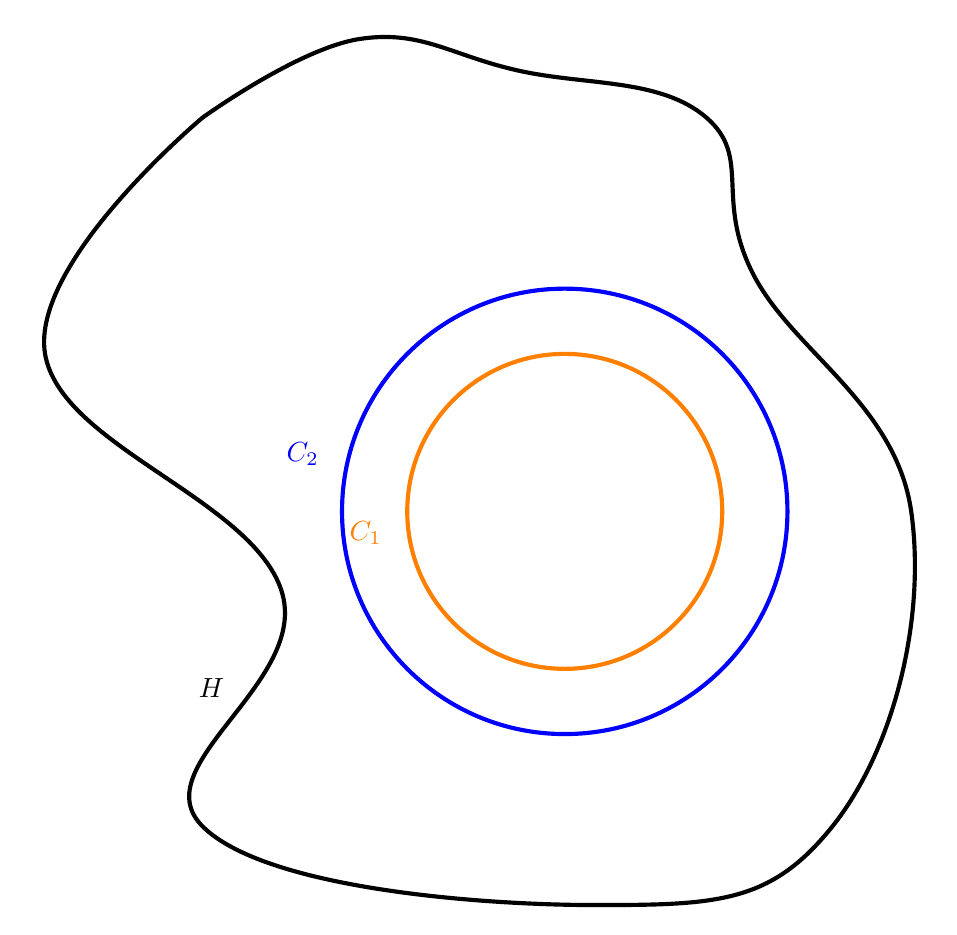
\begin{tikzpicture}[scale=2.0]
\path
(2.2,2) node[below left, text=black]{$H$};
\path
(2.8,3.5) node[below left, text=blue]{$C_2$};
\path
(3.2,3) node[below left, text=orange]{$C_1$};
\draw [black, line width = 1.5]  plot[smooth, tension=.7] coordinates {(2,5.5) (3,6) (4,5.8) (5.2,5.5) (5.5,4.5) (6.5,3) (6,1)(4.5,0.5) (2,1) (2.5,2.5) (1,4) (2,5.5)}; 
\draw[blue, line width = 1.5] (4.3 ,3) circle({sqrt(2)});
\draw[orange, line width = 1.5] (4.3 ,3) circle({sqrt(1)});
\end{tikzpicture}
\end{center}
\end{figure}
From the definition
$$d(x, C_1) = \inf \{ d(x, y) \qquad \textrm{s.t.} \qquad y \in C_1 \}$$
we have
$$4 \norm{x - \frac{P_{C_1}(x) + P_{C_2}(x)}{2}}^2 + \norm{P_{C_2}(x) - P_{C_1}(x)}^2 = 2(d(x, C_1)^2 + d(x, C_2)^2).$$
$C_1 \subseteq C_2$ are convex, then
$$\frac{P_{C_1}(x) + P_{C_2}(x)}{2} \in C_2,$$
then
$$\norm{x - (\frac{P_{C_1}(x) + P_{C_2}(x)}{2})}^2 \geq d(x, C_2)^2,$$
from which finally we obtain the desired inequality:
$$\norm{P_{C_2}(x) - P_{C_1}(x)}^2 \leq 2(d(x, C_1)^2 - d(x, C_2)^2).$$
\clearpage
\chapter{Operators}
\section*{Exercise $1$}
Let 
$$a(x) = \begin{cases}
			x \qquad if \quad x \in (0, \frac{1}{2}] \\
			0 \qquad if \quad x \in (\frac{1}{2}, 1]
		 \end{cases}$$
and consider the operator
$$T : L^2(0, 1) \rightarrow L^2(0, 1)$$
given by
$$Tf(x) = a(x) f(x), \qquad x \in (0, 1).$$
Show that $T \in \mathcal{L}(L^2[0,1])$ and compute $\norm{T}$.
\section*{Solution}
\begin{figure}[!ht]
\begin{center}
\begin{tikzpicture}[scale=2.0]
\draw[->] (-2.5,0)--(3.5,0) node[below]{$x$};   
\draw[->] (0,-1.5)--(0,1.5)  node[left]{$y$};
\draw[dashed] (0.5,-1.5)--(0.5,1.5);
\path
(0,0) node[below left]{$0$};
(0.5,0) node[below left]{$0.5$};
\path
(1.0,0) node[below left]{$1.0$};
\path
(1.0,1.0) node[below left]{$a(x)$};
\foreach \i in {0,0.1, 0.2,...,1.0} \draw (\i,-0.02)--(\i,0.02);
\draw[red, domain=0.:0.5, samples=100, variable=\x] plot ({\x}, {\x});
\draw[red, domain=0.5:1.0, samples=100, variable=\x] plot ({\x}, {0.});
\end{tikzpicture}
\end{center}
\end{figure}
$$f \in L^2(0, 1)$$
$$\norm{T f}_{L^2(0, 1)}^2 = \int_0^1 a(x)^2 f(x)^2 dx \leq \frac{1}{4} \int_0^1 f(x)^2 dx = \frac{1}{4} \norm{f}_{L^2(0,1)}^2$$
so that
$$\norm{T}_{\mathcal{L}(L^2(0,1))} \leq \frac{1}{2}.$$
Then we want to show that $\frac{1}{2}$ is the value of the norm, that is
$$\norm{T} = \frac{1}{2}.$$
We define
$$f_n(x) = \begin{cases}
			\sqrt{n} \qquad if \quad x \in [\frac{1}{2} - \frac{1}{n}, \frac{1}{2}], \qquad n \geq 2 \\
			0 \qquad \textrm{otherwise}
		   \end{cases}$$
\begin{figure}[!ht]
\begin{center}
\begin{tikzpicture}[scale=2.0]
\draw[->] (-2.5,0)--(3.5,0) node[below]{$x$};   
\draw[->] (0,-1.5)--(0,3.5)  node[left]{$y$};
\draw[dashed] (0.5,-1.5)--(0.5,3.5);
\path
(0,0) node[below left]{$0$};
\path
(0.5,0) node[below left]{$0.5$};
\path
(1.0,0) node[below left]{$1.0$};
\path
(1.0,1.0) node[below left]{$f_n(x)$};
\foreach \i in {0,0.1, 0.2,...,1.0} \draw (\i,-0.02)--(\i,0.02);
\draw[red, domain=0.:0.5, samples=100, variable=\x] plot ({\x}, {sqrt (2)});
\draw[red, domain=1./6:0.5, samples=100, variable=\x] plot ({\x}, {sqrt (3)});
\draw[red, domain=1./4:0.5, samples=100, variable=\x] plot ({\x}, {sqrt (4)});
\draw[red, domain=3./10:0.5, samples=100, variable=\x] plot ({\x}, {sqrt (5)});
\draw[red, domain=1./3:0.5, samples=100, variable=\x] plot ({\x}, {sqrt (6)});
\draw[red, domain=5./14:0.5, samples=100, variable=\x] plot ({\x}, {sqrt (7)});
\draw[red, domain=0.5:1.0, samples=100, variable=\x] plot ({\x}, {0.});
\draw[->] (0.1,-0.5)--(0.45,-0.5);
\path
(0.1, -0.6) node[below]{$\frac{1}{2} - \frac{1}{n}$};
\end{tikzpicture}
\end{center}
\end{figure}
$$\norm{f_n(x)}_{L^2(0,1)}^2 = \int_0^1 f_n(x)^2 = 1$$
Now we compute the norm of the image:
$$\norm{T f_n(x)}_{L^2(0,1)}^2 = \int_0^1 a(x)^2 f_n(x)^2 dx \geq \star$$
we can minor the integral with
$$\star \geq \int_{\frac{1}{2} - \frac{1}{n}}^{\frac{1}{2}} n(\frac{1}{2} - \frac{1}{n})^2 dx = (\frac{1}{2} - \frac{1}{n})^2 \rightarrow \frac{1}{4} \qquad \textrm{for} \quad n \rightarrow +\infty$$
so that
$$\norm{T}_{\mathcal{L}(L^2(0,1))} = \frac{1}{2}.$$
We can characterize the norm in various ways.
$$\norm{T}_{\mathcal{L}(L^2(0,1))} = \sup_{f \in L^2(0,1) \quad \norm{f}_{L^2} = 1} \frac{\norm{Tf}_{L^2(0,1)}}{\norm{f}_{L^2(0,1)}} \leq \frac{1}{2}.$$
We have shown that 
$$\norm{Tf_n(x)}_{L^2(0,1)}^2 \geq \frac{1}{4},$$
that is
$$\norm{T f_n(x)}_{L_2(0,1)} \geq \frac{1}{2},$$
but at the same time we have
$$\norm{T} \leq \frac{1}{2}$$
then
$$\norm{T f_n(x)} = \frac{1}{2}.$$
\clearpage
\section*{Exercise $2$}
Let $(f'_h)_{h \in \mathbb{N}} \in L^p$ for some $p$, with the following hypotheses:
\begin{itemize}
\item $(f'_h)_{h \in \mathbb{N}}$ is bounded in $L^p$ for some $p$;
\item $f_h(0)$ is bounded.
\end{itemize}
Show that $(f_h)_{h \in \mathbb{N}}$ is compact (relatively) in $(C([0,1]), \norm{\cdot}_{\infty}$.
\section*{Solution}
From the hypotheses we can suppose that
$$f_h(x) = f_h(0) + \int_0^x f'_h(y) dy \qquad x \in [0, 1].$$
Since we have to show the compactness in the set of continuous fuunctions we need to utilize the Ascoli-Arzel\`{a} theorem. \par
Let $C > 0$ constant. \par 
\textbf{Equiboundedness}
$$h \in \mathbb{N}, \qquad x \in [0, 1]$$
$$|f_h(x)| \leq |f_h(0)| + \int_0^x |f'_h(y)| dy \leq \star$$
using the hypothesis $2$ and the H\"{o}lder inequality
$$\star \leq C + \norm{f'_h}_{L^p(0,1)} x^{\frac{1}{p'}} \leq M$$
so that
$$|f_h(x)| \leq M,$$
that is $f_h$ is equibounded. \par   
\textbf{Equicontinuity}
$$x, y \in [0, 1], \qquad x < y$$
$$f_h(y) - f_h(x) \leq \int_x^y |f'_h(w)| dw \leq \star$$
using the H\"{o}lder inequality
$$\star \leq \norm{f'_h}_{L^p(0,1)}|y - x|^{\frac{1}{p'}}.$$
This shows that the fuunctions $f_h$ are equi-h\"{o}lder  with exponent $\frac{1}{p'}$, in particular they are eqicontinuous. \par   
Then from the Ascoli-Arzel\`{a} theorem they are relatively compact.

\end{document}